%%%%%%%%%%%%%%%%%%%%%%%%%%%%%%%%%%%%%%%%%
% University Assignment Title Page 
% LaTeX Template
% Version 1.0 (27/12/12)
%
% This template has been downloaded from:
% http://www.LaTeXTemplates.com
%
% Original author:
% WikiBooks (http://en.wikibooks.org/wiki/LaTeX/Title_Creation)
%
% License:
% CC BY-NC-SA 3.0 (http://creativecommons.org/licenses/by-nc-sa/3.0/)
% 
% Instructions for using this template:
% This title page is capable of being compiled as is. This is not useful for 
% including it in another document. To do this, you have two options: 
%
% 1) Copy/paste everything between \begin{document} and \end{document} 
% starting at \begin{titlepage} and paste this into another LaTeX file where you 
% want your title page.
% OR
% 2) Remove everything outside the \begin{titlepage} and \end{titlepage} and 
% move this file to the same directory as the LaTeX file you wish to add it to. 
% Then add \input{./title_page_1.tex} to your LaTeX file where you want your
% title page.
%
%%%%%%%%%%%%%%%%%%%%%%%%%%%%%%%%%%%%%%%%%
%\title{Title page with logo}
%----------------------------------------------------------------------------------------
%	PACKAGES AND OTHER DOCUMENT CONFIGURATIONS
%----------------------------------------------------------------------------------------

\documentclass[12pt]{article}
\usepackage[english]{babel}
\usepackage[utf8x]{inputenc}
\usepackage{amsmath}
\usepackage{hyperref}
\usepackage{minted}
\usepackage[]{algorithm2e}
\usepackage{graphicx}

\usepackage{wrapfig}

\usepackage{titleps}

\usepackage[colorinlistoftodos]{todonotes}
\usepackage{hyperref}

\usepackage{geometry}
\geometry{bmargin=2in}

\usepackage[colorinlistoftodos]{todonotes}

% \usepackage{titlesec}
% \newcommand{\sectionbreak}{\clearpage}

\textheight=250truemm \textwidth=160truemm 
\hoffset=-10truemm \voffset=-20truemm

\begin{document}

\begin{titlepage}

\newcommand{\HRule}{\rule{\linewidth}{0.5mm}} % Defines a new command for the horizontal lines, change thickness here

\center % Center everything on the page
 
%----------------------------------------------------------------------------------------
%	HEADING SECTIONS
%----------------------------------------------------------------------------------------

\textsc{\LARGE Ukrainian Catholic University}\\[1cm] % Name of your university/college
\textsc{\Large  Faculty of Applied Sciences}\\[0.5cm] % Major heading such as course name
\textsc{\large Computer Science Programme}\\[0.5cm] % Minor heading such as course title

%----------------------------------------------------------------------------------------
%	TITLE SECTION
%----------------------------------------------------------------------------------------
\vspace*{1cm}

\HRule \\[0.4cm]
{ \huge \bfseries Simultaneous Localization and Mapping }\\[10pt]
{\Large \bfseries Linear Algebra final project report}\\[0.4cm] % Title of your document
\HRule \\[1cm]
 
%----------------------------------------------------------------------------------------
%	AUTHOR SECTION
%----------------------------------------------------------------------------------------
\vspace*{1cm}

% If you don't want a supervisor, uncomment the two lines below and remove the section above
\Large \emph{Authors:}\\
Bohdan \textsc{Hlovatskyi}, Mykhailo \textsc{Pasichnyk}, Stefan-Yuriy \textsc{Malyk}\\[1cm] % Your name

%----------------------------------------------------------------------------------------
%	DATE SECTION
%----------------------------------------------------------------------------------------
\vspace*{1cm}
{\large May 2022 }\\[2cm] % Date, change the \today to a set date if you want to be precise

%----------------------------------------------------------------------------------------
%	LOGO SECTION
%----------------------------------------------------------------------------------------


\includegraphics[height=5cm]{UCU-Apps.png}\\[1cm] % Include a department/university logo - this will require the graphicx package
 
%----------------------------------------------------------------------------------------

\vfill % Fill the rest of the page with whitespace

\end{titlepage}

% ~\cite{Strang}

\tableofcontents


\begin{abstract}
SLAM or Simultaneous Localization and Mapping - the problem of constructing a map of an unknown environment, simultaneously tracking the object's location. SLAM algorithms utilize the data obtained from sensors, such as video camera, LIDAR etc to construct a 3-D model of the nearby objects and estimate the relative location of the tracking device itself. They are used in variety of fields: autonomous driving, robotics, augmented reality and much more. The algorithms that rely on video data are referred to as Visual SLAM. They obtain information by means of Computer Vision and different techniques of Signal Processing. In the following work we review available approaches along with the implementation of the chosen one by means of Python and \mintinline{python}{pyopencv} as our Linear Algebra course work. Source code: ~\cite{GitHub}.
\end{abstract}

\section{Introduction}

Visual SLAM is a family of algorithms that solve the problem of Simultaneous Localization and Mapping by means of Computer Vision. Depending on the type of input video stream there are different types of Visual SLAM:
\begin{itemize}
    \item Monocular SLAM. Such SLAM takes as an input video stream from a single RGB camera. The simplicity of the setup results in low costs, although implies some limitations, one being particularly significant. t Since a single frame is essentially a projection of a real-world scene to an image plane, we can construct environment map only to some scale factor. In other words, we cannot obtain the exact depth of featured points in an environment from a single image source, only approximate one using multiple images and translation movement.
    \item Stereo SLAM. Input video stream comes from two cameras. Cameras are positioned on some distance, called baseline, value of which is known beforehand. This allows to get the more accurate depth of the featured points. The limitation is that calibration and computation process is difficult usually requiring additional hardware to generate real-time outputs.
    \item RGBD. Specific kind of SLAM that gets the input data from RGBD camera - the one that included depth of objects within an image. The depth is computed by emitting light and calculating how much does it took for it to return back. However, this technology is relatively new. As a result the range is limited making it not suitable for outdoor use and price is higher, compared to approaches described above.
\end{itemize}


The pipeline of SLAM algorithms will usually look in the following way:
\begin{center}
    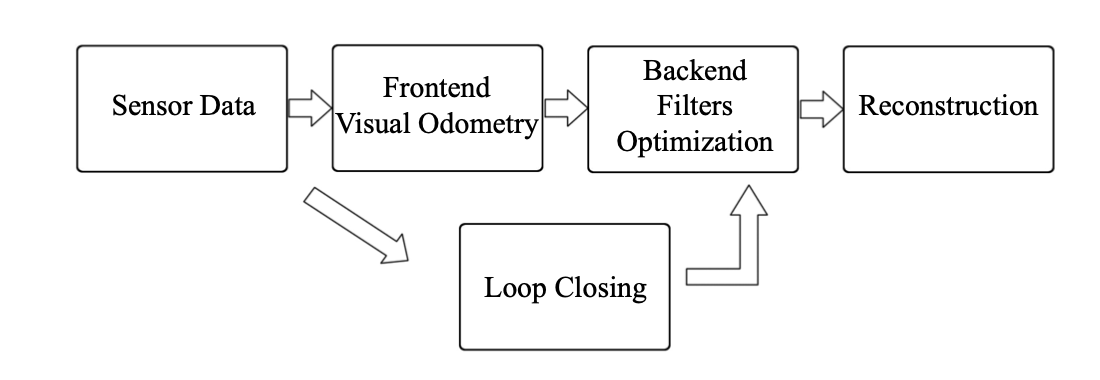
\includegraphics[height=4cm]{pipeline.png}\\[1cm]
\end{center}

In this work we are mainly interested in Frontend Visual Odometry, goal of which is to track the object that produces the source data and build non-optimized 3-D cloud map of the environment. Backend optimization and loop closing are powerful techniques to optimize the SLAM and get rid of the noise that brings a lot of inaccuracy in the SLAM algorithm. Those algorithm, such as Kalman and Particle filters, are beyond the scope of Computer vision and are related mainly to signal processing, thus won't be focused on here.

\section{Problem setting}

\subsection{Problem formulation}

With the given setting, we are interested mainly in two parts:
% 'change of state' kinda ambiguous 
% collecting landmarks is not a problem
\begin{enumerate}
    \item Modeling the object's motion. In an abstract setting this can be modeled as $x_{k} = f(x_{k - 1}, u_{k}, w_{k})$, where $x_{k}$ denotes a current position of an object, $x_{k - 1}$ - its previous position, $u_{k}$ - change of its state and $w_{k}$ - noise.  
    \item Gather information about the landmarks of a nearby environment. The observed data $z_{k, j}$ will then be described by this equation: $z_{k, j} = f(y_{j}, x_{k}, v_{k, j})$. Here $y_{j}$ - landmark point, $x_{k}$ - its coordinates, $v_{k, j}$ - noise of the observation.
\end{enumerate}

These two equation summarize the SLAM. For the Euclidean space the motion model can be expressed as the so-called special Euclidean Group: $$SE(3) = \{ T =
\begin{bmatrix}
    R    &  t      \\
    0^T  &  1      
\end{bmatrix} \in \mathbf{R}^{4x4} \},$$ where $R$ - rotation matrix, $t$ - translation vector. It allows to express state $a_{1}$ as $$a_{1} = R a_{0} + t.$$ Important note here is that we associate the state of an object with the location of camera that produces some input data.

\subsection{Camera model}

\begin{center}
    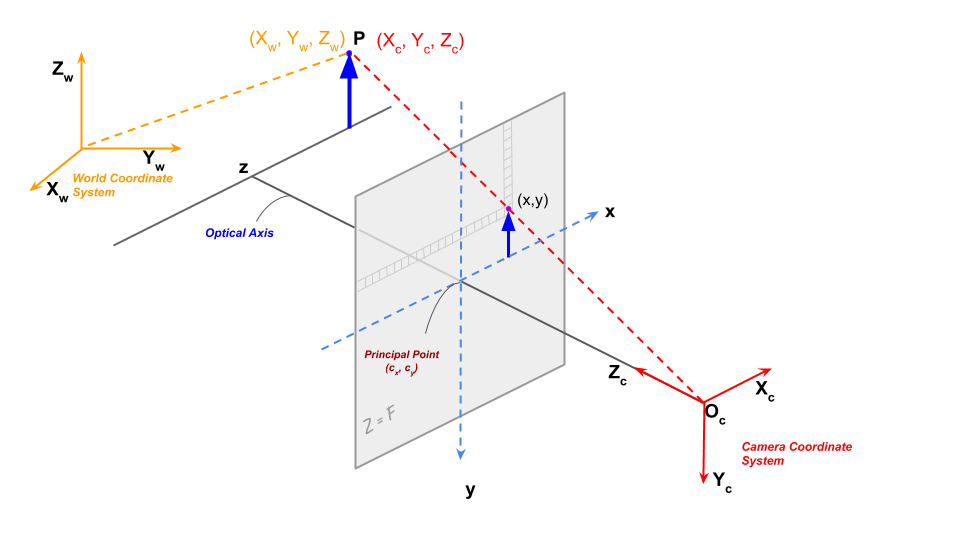
\includegraphics[height=5cm]{camera_model.png}
\end{center}

Any point in space can be represented by three coordinate systems:
\begin{itemize}
    \item The World Coordinate System - point \textbf{P} =  $(X_w, Y_w, Z_w)$. For example if our object is in a room we can threat floor as $x-y$ axis and a wall as $z$ axis
    \item The Camera Coordinate System - $(X_c, Y_c, Z_c)$ the same object in 3D space but from camera, where $X_c$ points to the right, $Y_w$ down and $Z_w$ towards the camera
    \item The point projection to the plane (image itself)
\end{itemize}
 
 The world and camera coordinate systems are related by the rotation matrix \textbf{R} and translation vector \textbf{t}. Thus
 
 \[
 \begin{bmatrix}
    X_c \\
    Y_c \\
    Y_c
\end{bmatrix}
=
\textbf{R}
 \begin{bmatrix}
    X_w \\
    Y_w \\
    Y_w
\end{bmatrix} 
+ \textbf{t}
\]
 We can rewrite statement above to make it more compact and call such  \begin{bmatrix}
    \textbf{R} | \textbf{t}
\end{bmatrix} 
matrix the \textbf{Extrinsic matrix}
\[
 \begin{bmatrix}
    X_c \\
    Y_c \\
    Y_c
\end{bmatrix}
=
 \begin{bmatrix}
    \textbf{R} | \textbf{t}
\end{bmatrix} 
\begin{bmatrix}
    X_w \\
    Y_w \\
    Z_w \\
    1
\end{bmatrix}
\]
Now that we have our point \textbf{P} in the camera coordinate system we can project it onto the plane. 

\begin{center}
    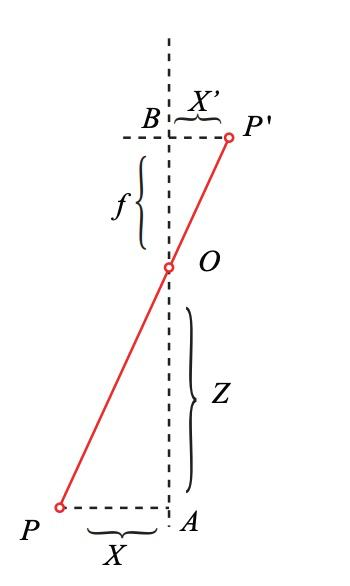
\includegraphics[height=4cm]{focal_length.jpg}
\end{center}

Our projected point $(x, y)$ can be found using following equations:\\
\begin{center}
    $x = f \cfrac{X_c}{Z_c}, y = f \cfrac{Y_c}{Z_c}$
\end{center}

where $f$ is the focal length of the camera. One important thing to mention is that the image \textbf{P} going though camera's optical center would be inverted. However, since usage of such camera would be inconvenient camera's software performs some transformation. Thus, this step could be omitted and we can stick to the equations above.
Next we construct such a matrix: \\
\[
\begin{bmatrix}
    x' \\
    y' \\
    z'
\end{bmatrix}
=
\begin{bmatrix}
    f & 0 & 0\\
    0 & f & 0 \\
    0 & 0 & f \\
\end{bmatrix}
\begin{bmatrix}
    Y_c \\
    X_c \\
    Z_c \\
\end{bmatrix}
\]
It would be referred as the \textbf{Intrinsic Matrix}.
Another important observation to make is that the optical center of the camera could be shifted from the origin of the camera coordinate system. Thus we need to modify the Intrinsic matrix as such:\\
\[\textbf{K} = \begin{bmatrix}
    f & 0 & c_x\\
    0 & f & c_y \\
    0 & 0 & f \\
\end{bmatrix}\]
Combining all of the above we can get coordinates of the object on our image $(u,v)$:\\
\[
\begin{bmatrix}
    u' \\
    v' \\
    w'
\end{bmatrix}
=
\begin{bmatrix}
    f & 0 & c_x\\
    0 & f & c_y \\
    0 & 0 & f \\
\end{bmatrix}
\begin{bmatrix}
    Y_c \\
    X_c \\
    Z_c \\
\end{bmatrix}
\]
where 
\begin{center}
    $u = \cfrac{u'}{w'}, v = \cfrac{u'}{w'}$
\end{center}

\subsection{Feature detection}
Firstly let define what a feature is. A feature is a some pattern in the image which has the following proprieties:
\begin{enumerate}
    \item {\bf Repeatability}: The same feature can be found in different images.
    \item {\bf Distinctiveness}: Different features have different expressions.
    \item {\bf Efficiency}: In the same image, the number of feature points should be far smaller than the number of pixels.
    \item {\bf Locality}: The feature is only related to a small image area.
\end{enumerate}

Historically there were 3 most popular approaches in algorithms of feature detection:
\begin{enumerate}
    \item {\bf  SIFT} (Scale-Invariant Feature Transform) : is one of the most classic. It is fully consider the changes in illumination, scale, and rotation during the image transformation, but is so calculating expensive, so rarely used in SLAM.


    \item {\bf FAST} : is extremely fast to compute. To understand its drawbacks, one should understand its algorithm in general. It selects a  pixel $p$ in the image, assuming its brightness as $I_p$. Then it sets a threshold $T$ (for example, $20\%$ of $I_p$). Afterwards it selects the 16 pixels on a circle with a radius of 3 and a center $p$. If there are consecutive $N$ points on the selected circle whose brightness is greater than $I_p+T$ or less than $I_p−T$ , then the central pixel $p$ can be considered a feature point. $N$ usually takes 12, which is {\br FAST-12}. Also $N$ could be 9 / 11 / etc, with respective names of FAST.
    \begin{center}
        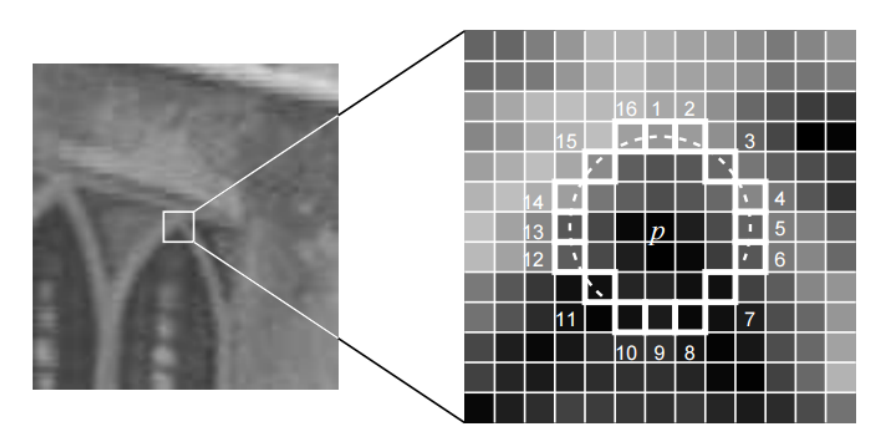
\includegraphics[height=3.5cm]{FAST_example.png}\\[1cm]
        [Fig 1] : Illustration of of FAST algorithm 
    \end{center}

    Clearly, such algorithm has an problem, that the detector does not have descriptors (fixed pattern, which try to find). Also, as it has fixed the radius of the circle = 3, there is a scaling problem.
    
    \item {\bf OBR}  (Oriented FAST and Rotated BRIEF) : it solves both mentioned problem of FAST, by adding the description of scale and rotation. In addition, it uses the extremely fast binary descriptor BRIEF. The scale invariance is achieved by the image pyramid and detect corner points on each layer. In terms of rotation, we calculate the gray centroid of the image near the feature point. The so-called centroid refers to the gray value of the image block as the center of weight. Then connect the geometric center $O$ and the centroid $C$ of the image block to get a direction vector $\overrightarrow{OC}$, so the direction of the feature point can be defined as: $\theta = arctan(\frac{m_{01}}{m_{10}})$.

\end{enumerate}

Due to the consideration of rotation and scaling, the ORB performs well under translation, rotation, and scaling. Meanwhile, the combination of FAST and BRIEF is very efficient, which makes ORB features very popular in real-time SLAM. Despite this, out tests showed that it is not enough for the requirement of being real-time in our implementation as we developed our SLAM via Python, thus we choose to use combination of improved BRIEF taken from the ORB algorithm and simple feature detection algorithm - Harris corner detection.

\subsection{Harris Corner Detector}

\subsection{BRIEF}

After extracting the Oriented FAST key points, we calculate the descriptor for each point. ORB uses an improved BRIEF feature description. BRIEF is a binary descriptor. Its description vector consists of many zeros and ones, which encode the size relationship between two random pixels near the key point (such as p and q): If p is greater than q, then take 1, otherwise take 0. If we take 128 such p, q pairs, we will finally get a 128-dimensional vector consisting of 0s and 1s. The BRIEF implements the comparison of randomly selected points, which is very fast. Since it expresses in binary, it is also very convenient to store and suitable for real-time image matching. The original BRIEF descriptor does not have rotation invariance, so it is easy to get lost when the image is rotated. The ORB calculates the direction of the key points in the FAST feature point extraction stage. The direction information can be used to calculate the Steer BRIEF feature after the rotation so that the ORB descriptor has better rotation invariance. 

% \section{Features matching}
% After we define features in two frames we should match them together, to detect motion between them. Come on, it's easy! Just do it by yourself.

\subsection{Epipolar geometry}

The object motion can be found from the correspondence between two consecutive video frames. 
\begin{center}
    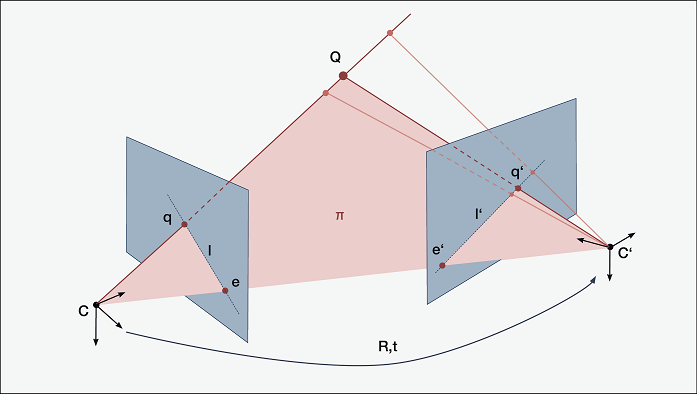
\includegraphics[height=5cm]{nc.png}\\[1cm]
\end{center}

According to the camera model, each of the landmarks $Q$ will be projected onto 2-D plane of pixels as $q, q^{\prime}$. Motion, described by the rotation matrix $R$ and transformation vector $t$ can be reproduced than via Epipolar constraint. 

Pixel points $q, q^{\prime}$ are described by the following equations:
\begin{equation}
    \begin{cases}
      s_{1} p_{1} = K P\\
      s_{2} p_{2} = K(RP + t)
    \end{cases}\,.
\end{equation}

As was discussed in the setting, due to the limitations of the approach, we can represent the points only to some constant factor. Moreover, it is worth mentioning that $p_{1}, p_{2}$ will be the points matched by the feature matcher.

To find the coordinates on the normalized plane of two pixels, we can simply take the inverse of the matrix representing a camera:
$x_{1, 2} = K^{-1}p_{1, 2}.$ Then the equation above can be rewritten as $x_{2} = Rx_{1} + t.$ This can be further transformed into $$p_{2}^{\italic{T}} K^{-T} t \times R K^{-1} p_{1} = 0.$$ This equation is referred to as epipolar constraint. For the sake of simplicity, the notions of Fundamental and Essential matrices are introduced:
\begin{equation}
    \begin{cases}
      E = t \times R\\
      F = K^{-T} t \times R K^{-1}\\
      x_{2}^{\italic{T}} E x_{1} = 0\\
      p_{2}^{\italic{T}} F p_{1} = 0
    \end{cases}\,.
\end{equation}
% is essential matrix ?
It is clear that usage of Essential matrix will make the calculations more accurate, as it uses precomputed calibration parameters for the camera. 
The process of camera pose estimation can then be summarized as:
\begin{enumerate}
    \item Find $E$ or $F$ from the known pixel positions.
    \item Find $R$, $t$ based on those matrices.
\end{enumerate}

In practice, the Essential matrix is found via Eight-Point algorithm and then $R, t$ are found via SVD and triangulation to get the result that would satisfy the constraints given by the known projections of landmarks.
Let SVD decomposition of \textbf{E} be:
$$
E = U \Sigma V^\top
$$

\begin{equation}
    \begin{cases}
        R = U R_{Z(\pm  \frac{\pi}{2})} V^{T}\\
        t = U R_{Z(\pm  \frac{\pi}{2})} \Sigma U^{T}
    \end{cases}\,.
\end{equation}

\subsection{RANSAC}


\subsection{Triangulation}

The second goal of SLAM is to estimate the relative positions of the feature points. Knowing the relative position of the camera and the relative positions of those featuer points, we can reconstruct their global coordinates and construct the feature map of the environment. 

\begin{center}
    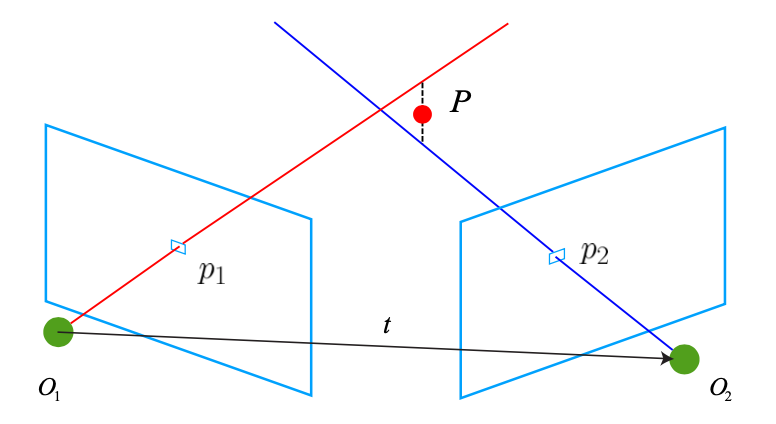
\includegraphics[height=5cm]{triangulation.png}\\[1cm]
\end{center}

From the epipolar constraint: $s_{2} x_{2} = s_{1} R x_{1} + t$. Here $x_{1, 2}$ - normalised coordinates (coordinates in the pixels' plane) of two feature points. Knowing $R, t$, we can now calculate $s_{1, 2}$ that will represent the 'depth' of a pixel. 

\begin{equation}
    s_{2} x_{2} \times x_{2} = 0 = s_{1} x_{2} \times R x_{1} + x_{2} \times t,
\end{equation}
which can be solved for $s_{1}$. Geometrically, we seek to find a 3D point on the ray $O_{1}p_{1}$ to make its projection close to $p_{2}$.
\pagebreak

\section{Overview of approaches}
As was mentioned earlier, there exist different types of SLAM algorithms that depend on different types of the input video stream. Though as we are focusing particularly on the visual SLAM in this work, we would consider different approaches to the SLAM problem from the perspective of Computer Vision:

\begin{itemize}
    \item The most popular implementation of visual SLAM is OpenVSLAM available open-source. It utilises notions of gloval and local key frame maps. For the local map it finds points via triangulation and for the global one uses pose-graph optimization. It also contain a global optimization module, which optimizes mathcing against global map. ~\cite{OpenVSLAM}
    \item Interesting to mention is the approach proposed by the ORB-SLAM \cite{ORB_SLAM}.
   % don't like the sentence, need to rewrite
    The project combines some of the fastest and most efficient algorithms resulting in being one of the most complete and reliable solutions. Some of the notable features and advantages are listed below:
    \begin{itemize}
        \item Same features are used for multiple tasks e.g tracking, mapping, localization, loop-closing. This approach allows real-time performance without using additional hardware.
        \item Could be operated in large environments thanks to a covisibility graph, which consists of keyframes as nodes and edges between nodes that have as least 15 map points 
        \item Real time loop is performed with an Essential Graph, a subgraph of covisibility graph that has at least 100 matching points
        \item The authors use beg-of-words representation of encoded descriptors for each of the feature points in order to optimise the process of feature matching against the stored feature map.
    \end{itemize} It has also a logical continuation as ORB-SLAM 2, which introduced ability to work with stereo and RGB-D input data. ~\cite{ORB_SLAM2}
    \item Speaking of the camera calibration, the classical approach to it is using a chess board photos from different perspective in order to estimate the intrinsic parameters. However the limitation of this approach is the fact that you cannot recover the intrinsic parameters having the video without direct access to the camera itself. Therefore it is worth mention some of the work focusing on the camera calibration using planar scenes. ~\cite{Self_Calibration}. It uses homography-based self-calibration to obtain required parameters. Authors prove that this type of calibration is as accurate as classical approach. Moreover planar scenes could be give  more robust result than when using an arbitrary scene.
    \item The research in the SLAM field is being actively maintained as technology have seen some success and made big technological companies interested. The problem is that many researches implement their own SLAM structure making it hard to test particular parts of the implementation, compare trade offs of different approaches and testing results. Thus the need of generalized SLAM frameworks emerged to ease research work and ideas exchange. The good example of such framework is GSLAM expressed in the cited paper. ~\cite{GeneralFramework}. It provides open-source, plugin based approach alongside with universal benchmarking solution.
\end{itemize}

\pagebreak
\section{Implementation}

The algorithm was implemented in Python mainly via pyopencv. The visualizer of the SLAM was written via OpegGL. For the feature extraction the Harris corner detector and BRIEF corner descriptor were used due to its computational efficiency. Feature matching was done in KNN manner because limitation on the number of features was only several hundreds. Because on the validation and test videos we had camera intrinsics, we used Essential matrix to recover rotation and transformation between two frames. The last step was to conduct triangulation so to get the 3-D coordinates of feature points. Demonstration of the algorithm can be found on Github or YouTube.

\vspace{5mm} %5mm vertical space

\begin{algorithm}[H]
	\KwData{stream of video frames}

	$init()$ /* make all the necessary initialization of visualizer and SLAM engine */ \;
	
	$prev \gets \begin{bmatrix}
	    1 & 0 & 0 & 0 \\ 0 & 1 & 0 & 0 \\ 0 & 0 & 1 & 0 \\ 0 & 0 & 0 & 1
	\end{bmatrix}$\;
	
	$currentFrame \gets None$\;
	$prevKeyPoints \gets None$\;
	
	\While{true}{
		$cur \gets getFrame()$\;
		
		$keyPoints \gets getFeatures(currentFrame)$\;
		
		\eIf{$prevKeyPoints$ is None}{
            $prevKeyPoints \gets keyPoints$\;
            continue\;
		} {
		    $matches \gets getMatches(keyPoints, prevKeyPoints)$\;
		    $E \gets recoverEssentialMatrix(method=RANSAC, matches)$\;
		    $R, t \gets recoverPose(E)$\;
		    
		    $points \gets trinagulate(matches , prevFrame, cur)$\;
		    
		    /* store all the necessary info */\;
		    $poses.append([R, t])$\;
		    $pointMap.extend(points)$\;
		    
		    \;
		    /* update all the values */\;
		    $tmp \gets cur$\;
		    $cur \gets prev @ cur$\;
		    $prev \gets tmp$\;
		    
		    $prevKeyPoints \gets keyPoints$\;
		}

	}
	\caption{General algorithm of SLAM}
\end{algorithm}

\pagebreak
\section{Experiments}
Experimentation was conducted on publicly available Kitty dataset~\cite{Kitty}. It was collected via a standard station wagon with two high-resolution color and grayscale video cameras and is widely used in testing of different SLAM approaches. Accurate ground truth is provided by a Velodyne laser scanner and a GPS localization system. As we are working only with monocular SLAM we took only the video from the first camera to conduct testing. Moreover, the dataset also provided calibration data for cameras, which took out the need of researching of obraining camera calibration from a given video source, which is completely another topic.

Evaluation was conducted on a small subset of the provided dataset, due to lack of computational resources, to be more specific - {\bf 2011-09-26-drive-0095'}. 
To measure metrics, we used open-source librbary for SLAM researchers - {\bf evo} ~\cite{Evo}. It contains tools to measure absolute and relative errors, whether matrices that describe poses conform to SE(3) restriction and many more. 
\vskip 1cm
The algorithm was implemented in Python via pyopencv. The visualizer of the SLAM was written via OpegGL. For the feature extraction the ORB was used due to its computational efficiency. Feature matching was done in brute-force manner because limitation on the number of features was only several hundreds. Fundamental matrix was then constructed as we lack the camera parameters for the test video. 

\begin{wrapfigure}{l}{0.4\textwidth}
    \centering
    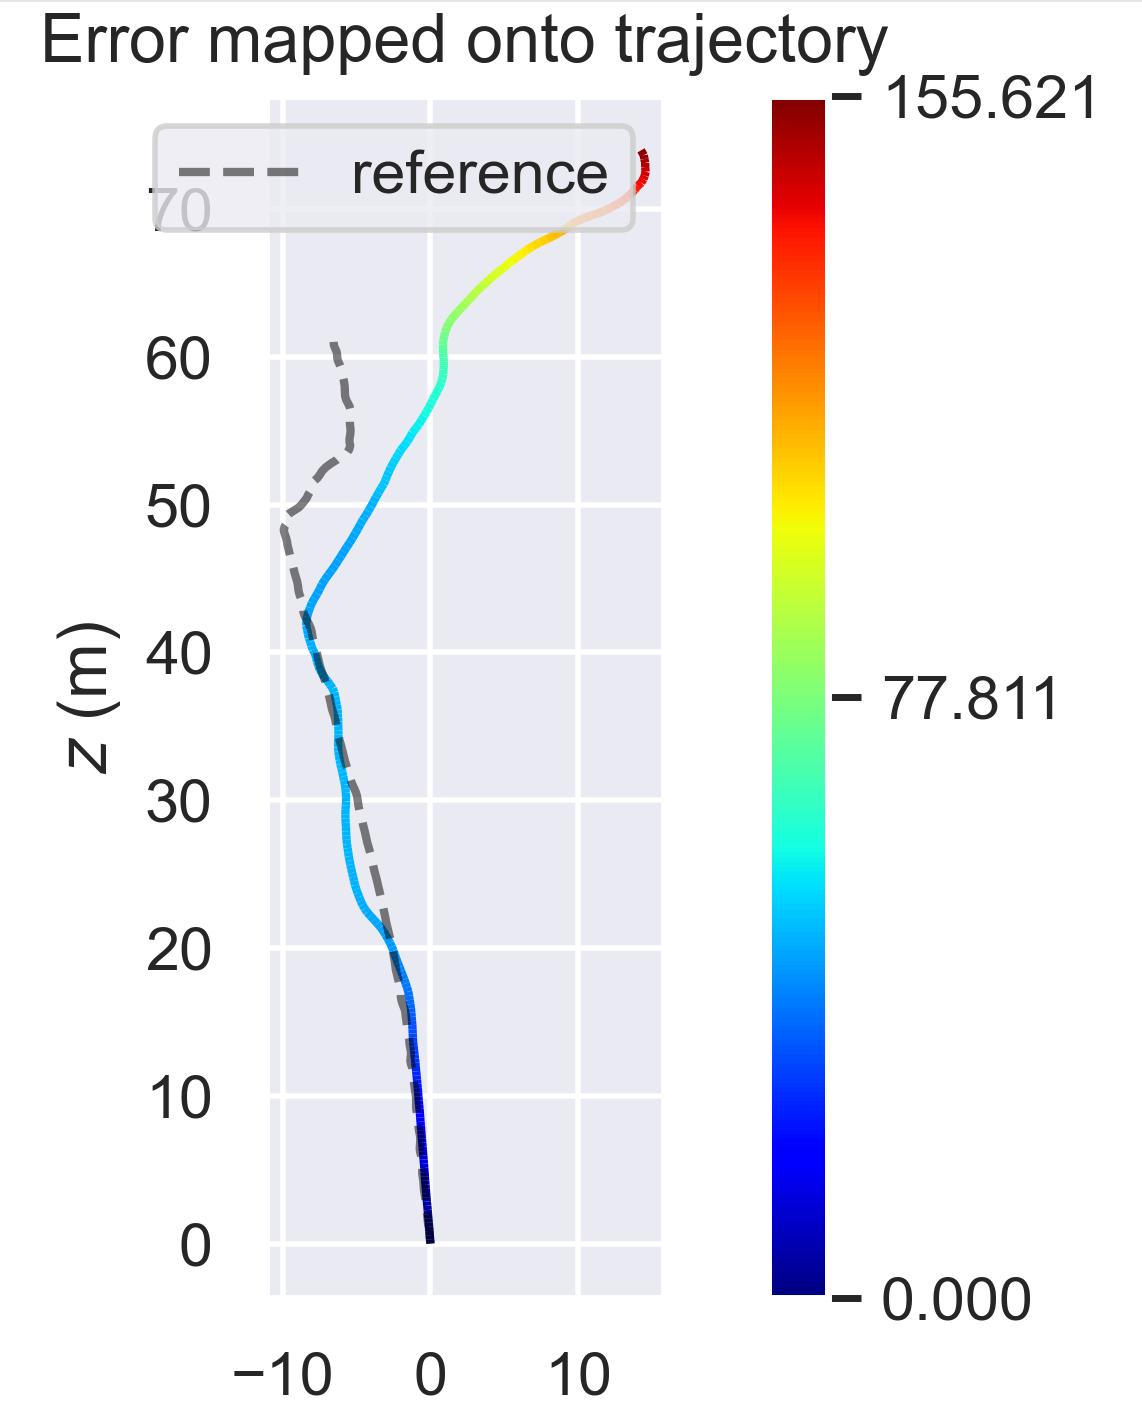
\includegraphics[width=0.4\textwidth]{results/error_mapped.png}
\end{wrapfigure}

We mainly focused no {\bf RPE} - relative pose error, which allows to investigate the local consistency of a SLAM trajectory, which is the most interesting metric for us as out SLAM is not stable on long distances because due to lack of backend optimizers, which result in a huge absolute error.

RPE compares poses along estimated and reference trajectory. It bases on delta pose difference ~\cite{ErrorMeasurement}: 
\begin{equation}
E_{i, j} = (P^{-1}_{ref, i} * P_{ref, j})^{-1} * (P^{-1}_{est, i} * P_{est, j})^{-1} \in SE(3);
\end{equation}

\begin{equation}
    RPE_{i, j} = ||E_{i, j} - I_{4 x 4}||_{F}
\end{equation}

It is easy to notice the drift that the system suffers from - the reason for that is that the error accumulates constantly and we could not get rid of it without some non-linear optimizer, which was not in the focus of this project.

To see the drift ever more clearly, we would decompose the position into set of (x, y) coordinates:

\begin{figure}[h]
\caption{Estimated y coordinate (in meters) against ground truth over iterations.}
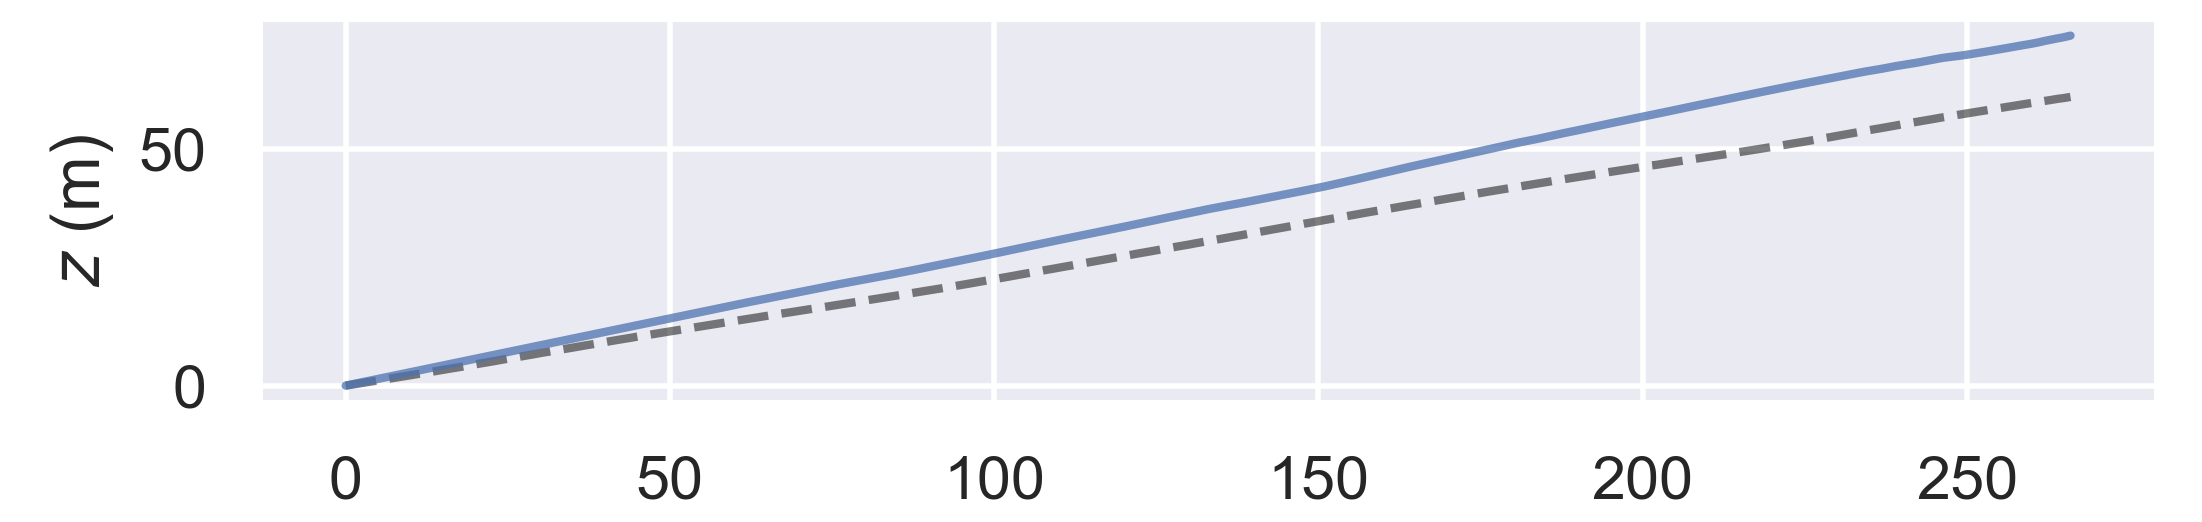
\includegraphics[height=5cm, width=15cm]{results/y_coord_over_time.png}
\end{figure}

\begin{figure}[!htb]
\caption{Relative error of estimated rotations.}
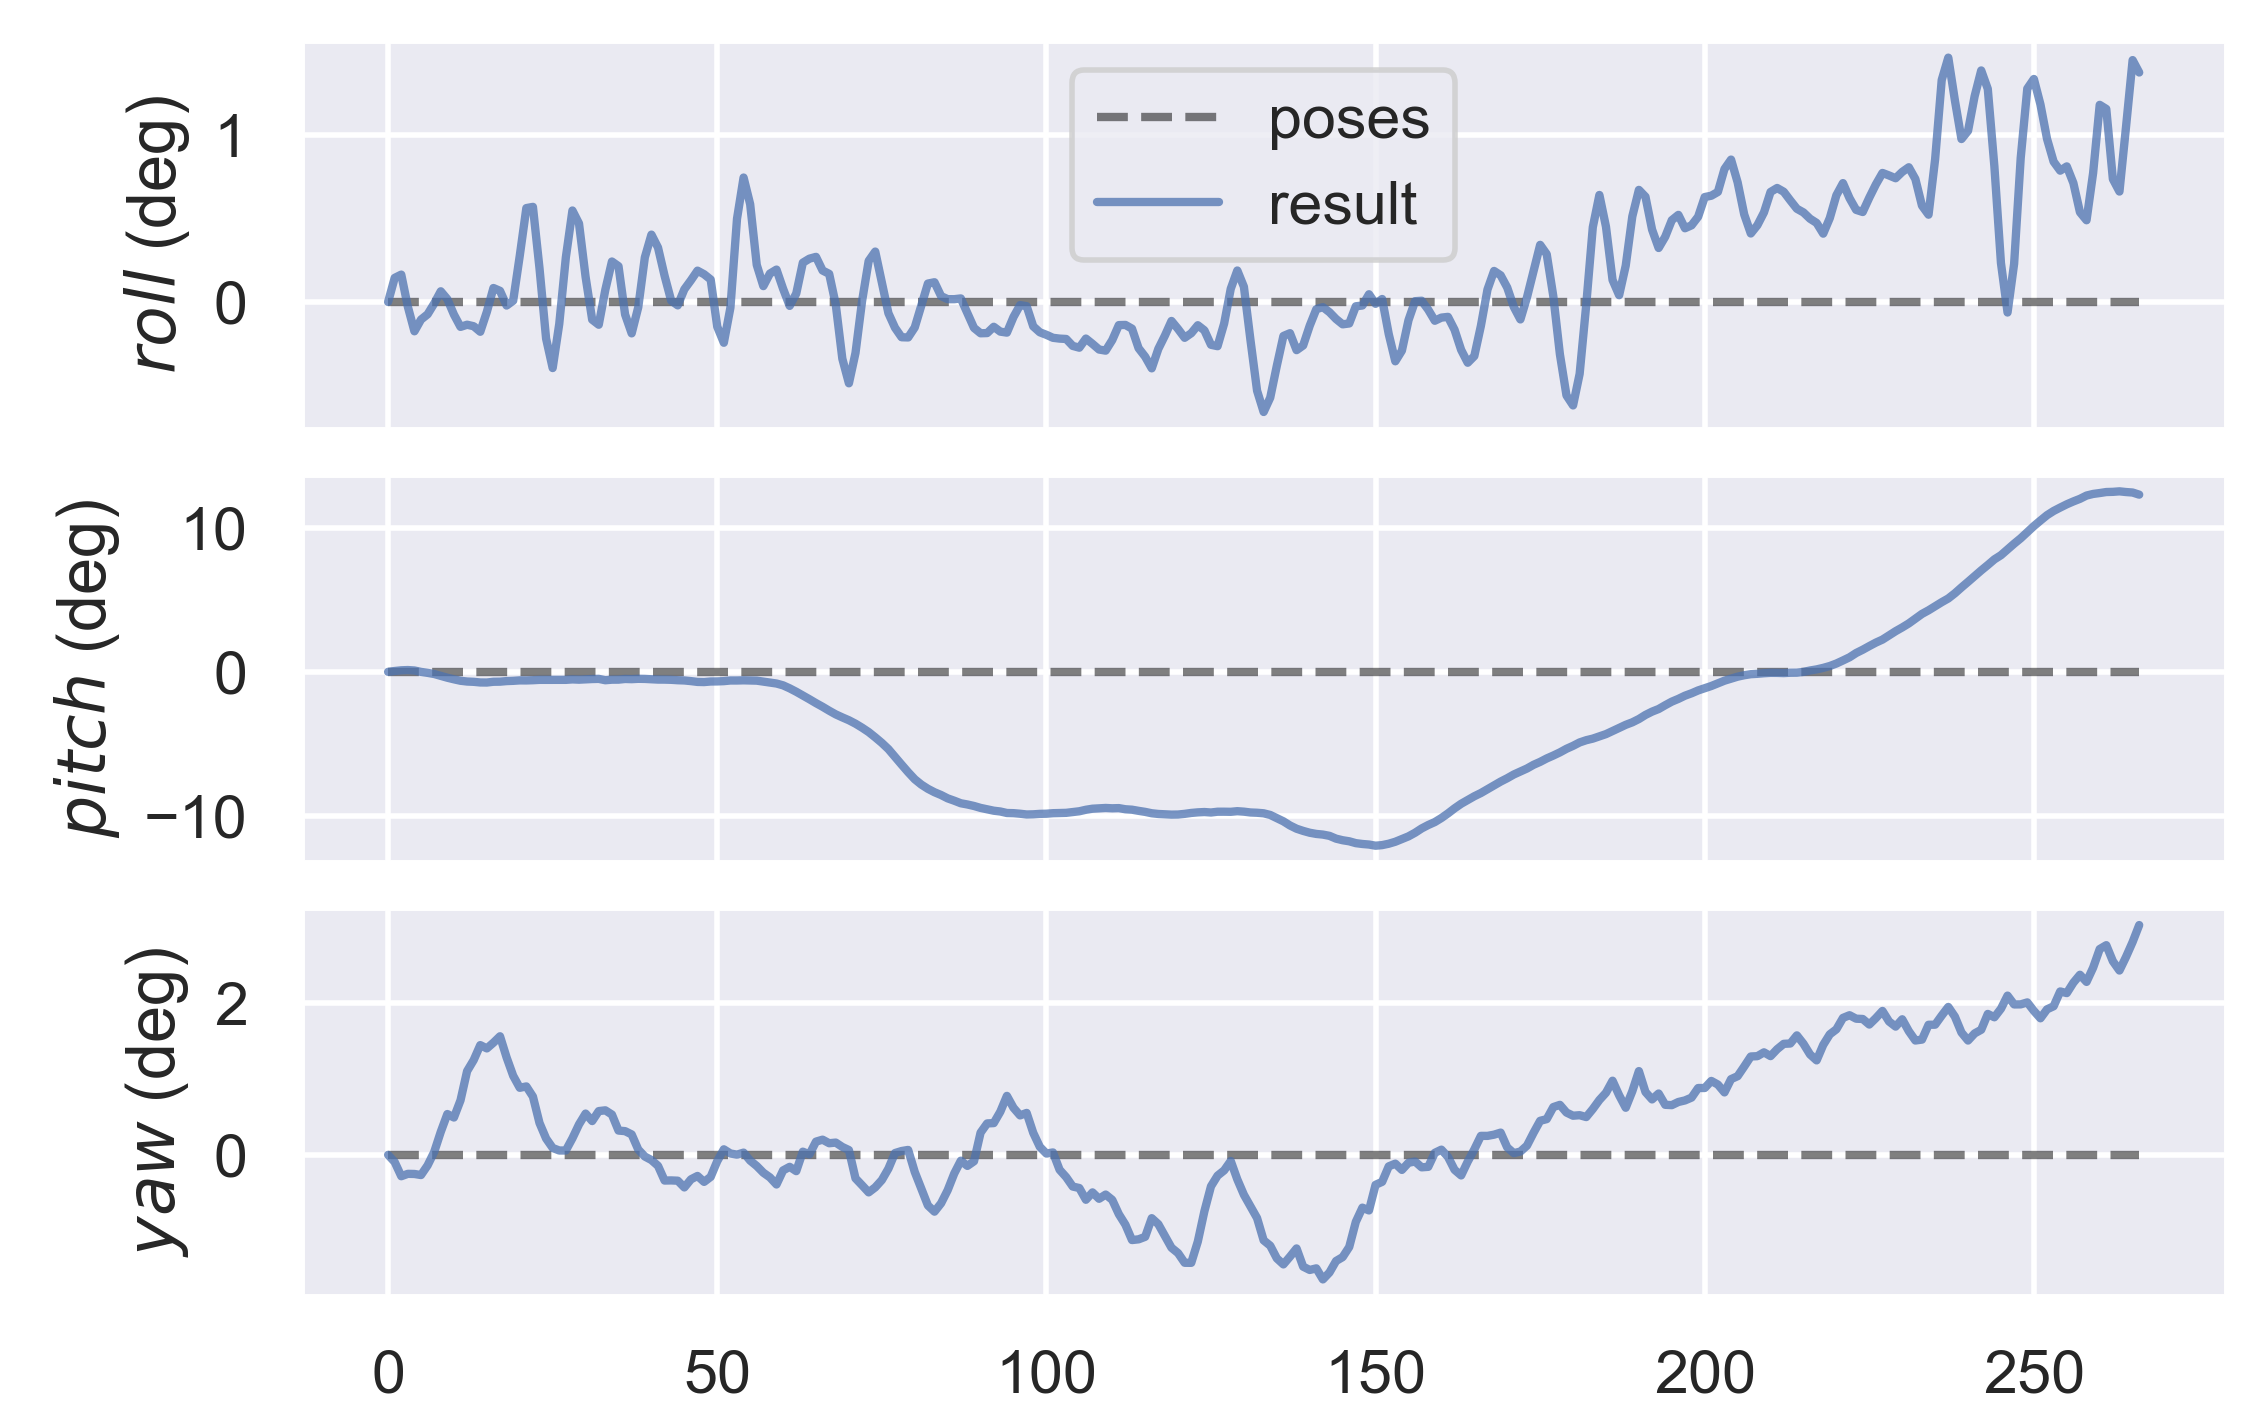
\includegraphics[height=9cm, width=15cm]{results/rotation.png}
\end{figure}

\begin{figure}[!htb]
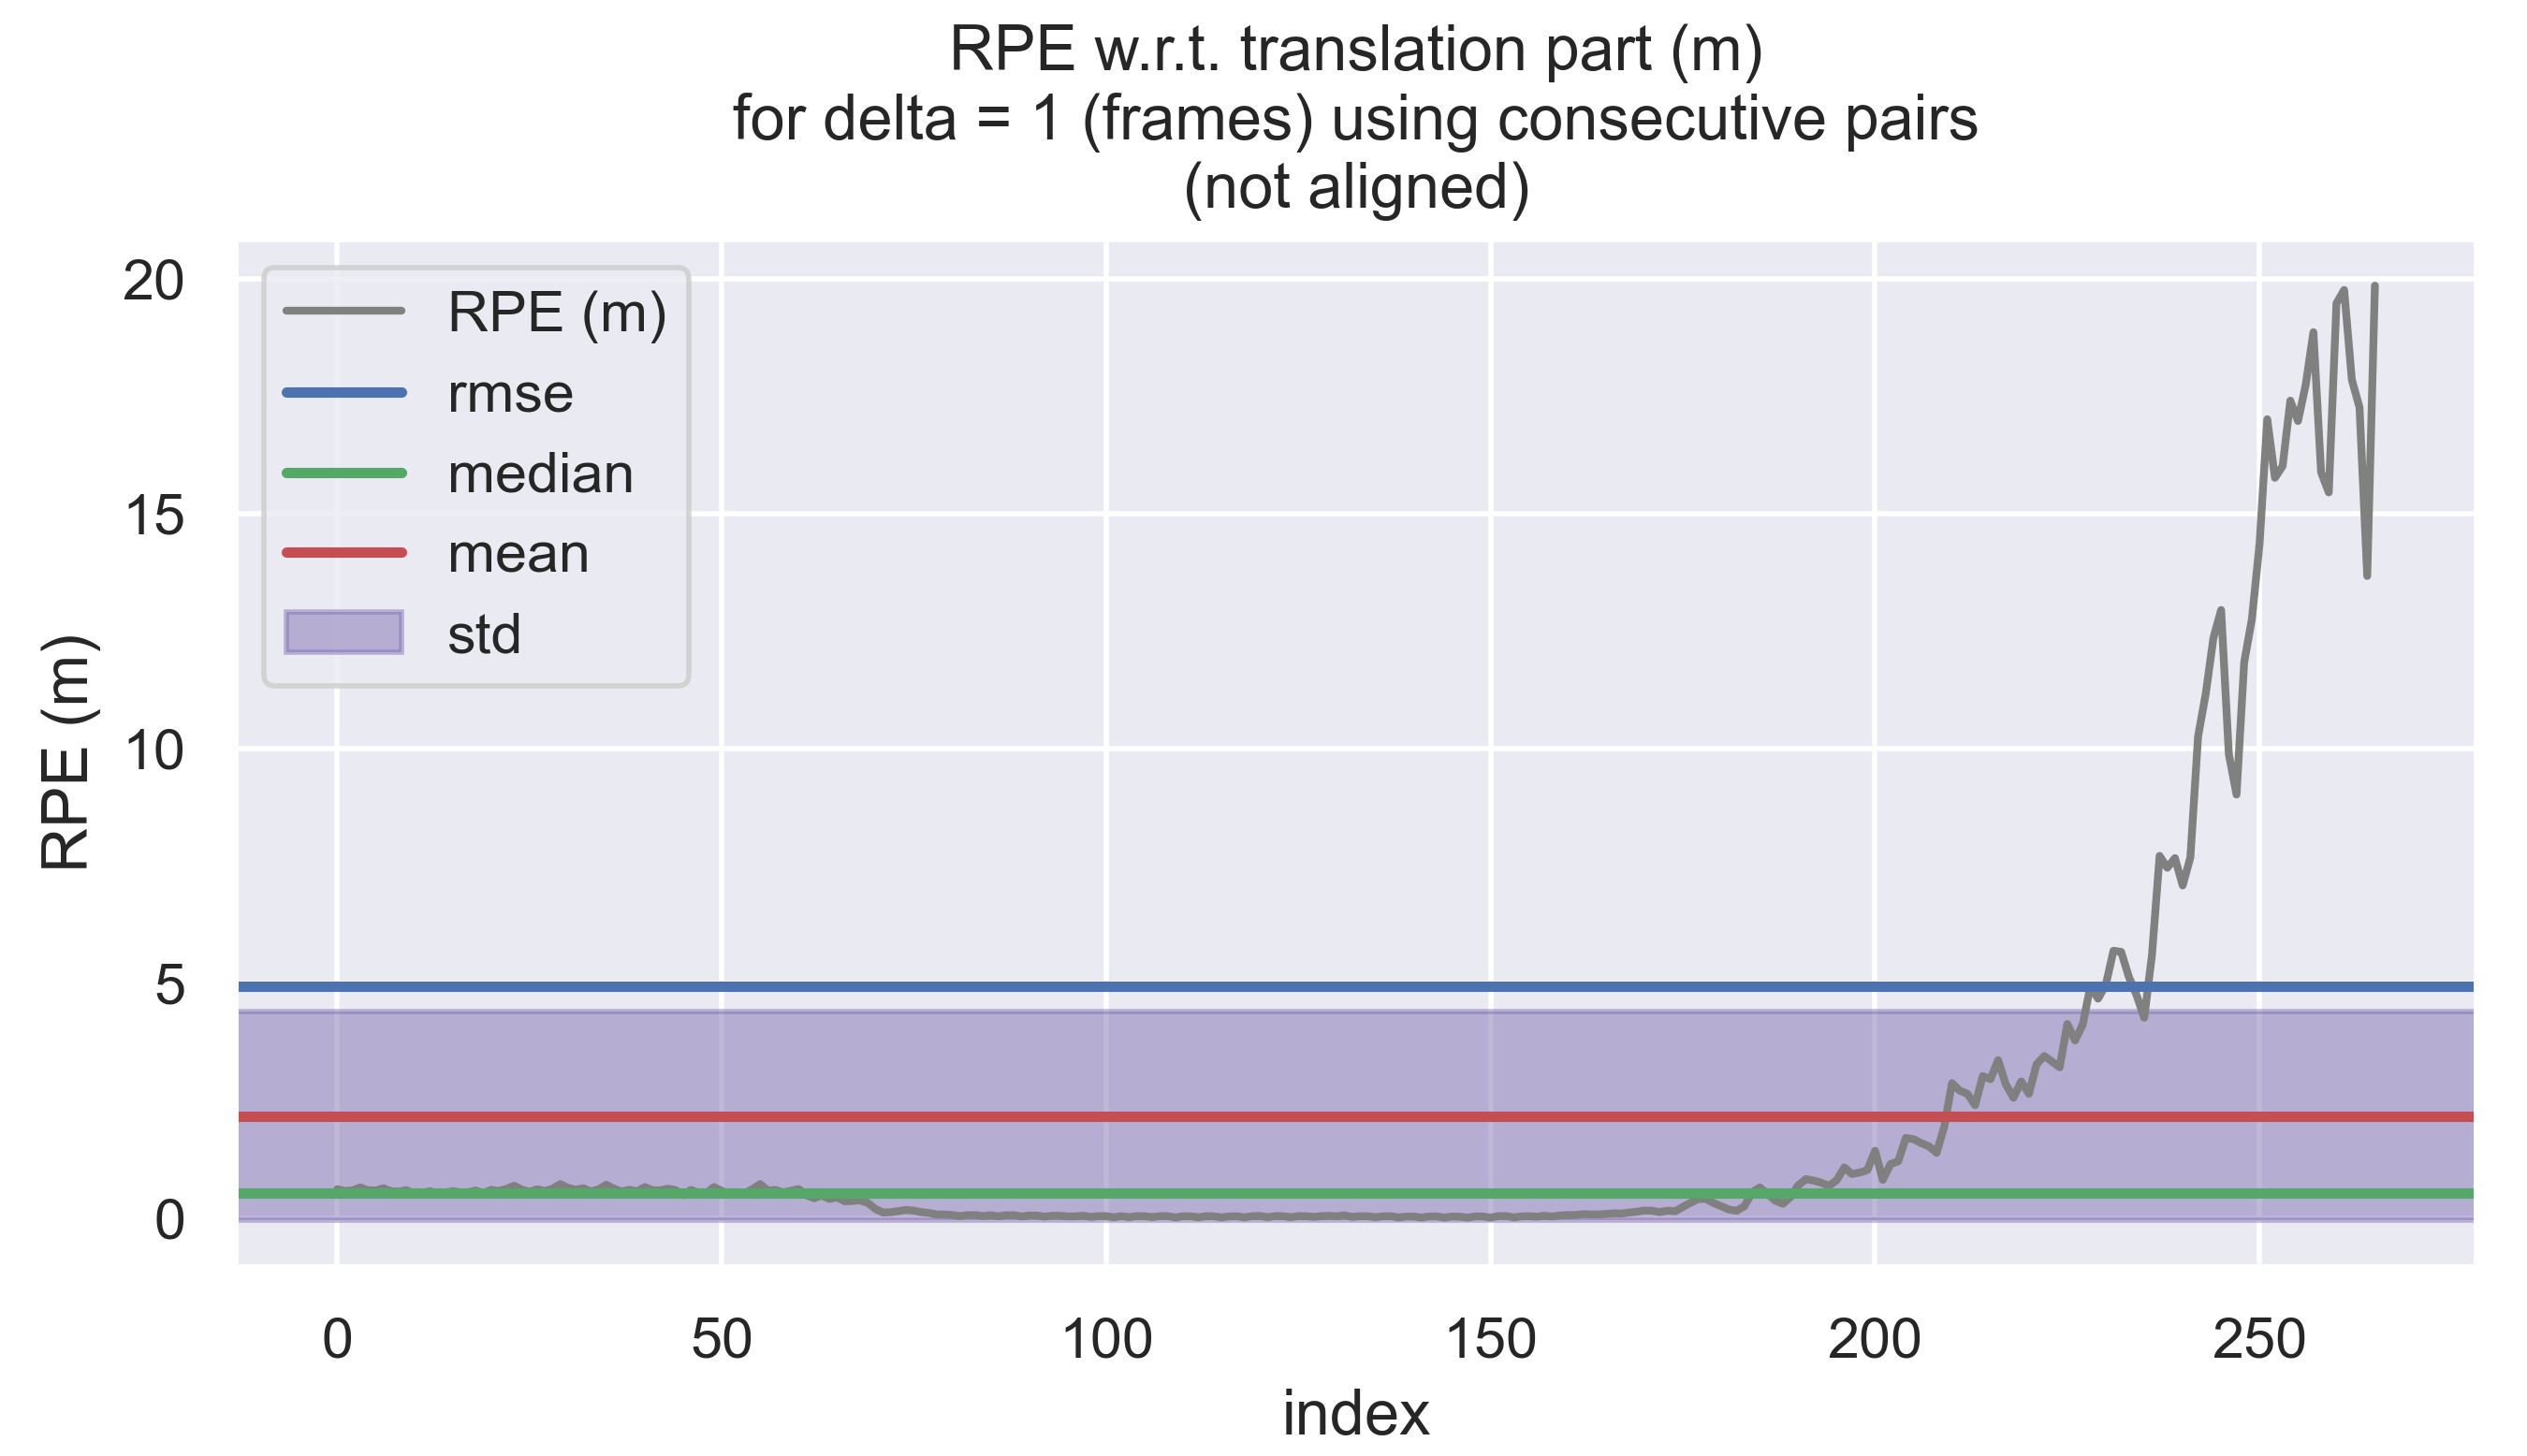
\includegraphics[height=9cm, width=15cm]{results/rel_err.png}
\end{figure}

\pagebreak
\section{Limitations}

Monocular SLAM is the simplest SLAM possibles, thus it possesses many limitations. The most prominent from them are the following:

\begin{enumerate}
    \item Main limitation of monocular SLAM is the fact that it can determine translation only to some constant factor, as while we projecting world onto image plane we lose the information about depth of objects that we see. To overcome this problem, one may use different type of camera - RGBD (measures depth as well) or different type of algorithm - Stereo SLAM - the one that takes images simultaneously captured from two or more cameras. 
    \item Triangulation is only possible if the enough amount of translation is present. If the amount of translation is small, pixel's change would result in big depth uncertainty. On the other hand, if translation is too big, the algorithm may fail to match the features. This problem will be especially seen in cases of so-called pure rotation, when there is no translation. Though in not so extreme cases, there are means to make this problem less visible - delayed triangulation etc.
    \item Assumption about static sight of view brings a lot of limitations as well.  For instance, the algorithm cannot be applied to autopilots as the moving object would make it think that the camera has moved. 
\end{enumerate}

\section{Conclusions}
In this work we developed a Monocular SLAM engine which allows us to track object given input video source from a single camera. It gives adequate results, speaking in terms of relative pose error, in short terms, though suffers from error accumulation over time. Basing on reviewed literature, back end optimizers, such as Extended Kalman Filter or Bundle Adjustement, which utilizes non-linear optimizers to make the error of projections of discovered features points in world coordinates as small as possible, could greatly improve the overall quality of SLAM and get rid of those accumulated errors. Sadly, this part if more connected with signal processing and non-linear optimization rather than with Linear Algebra thus we did not focus on that in this work. Speaking about the further work, we would propose to implement one of those optimizers to make SLAM more accurate. We also see this project as a great foundation for further research for us - combined with deep learning, 3-D map and poses obtained by SLAM could greatly influence the field of reinforcement learning for robots. 


\pagebreak
\appendix
\begin{thebibliography}{10}

\bibitem{GitHub} \url{https://github.com/bohdanhlovatskyi/OhISee}
\bibitem{Testing_Data} \url{http://www.cvlibs.net/datasets/kitti/eval_odometry.php}

\bibitem{ORB_SLAM} \url{http://webdiis.unizar.es/~raulmur/MurMontielTardosTRO15.pdf}
\bibitem{ORB_SLAM2} \url{https://128.84.21.199/pdf/1610.06475.pdf}

\bibitem{Camera_Calibration} \url{https://www.microsoft.com/en-us/research/wp-content/uploads/2016/02/tr98-71.pdf} 

\bibitem{Self_Calibration} \url{https://users.aalto.fi/~kannalj1/publications/wacv2016.pdf}

\bibitem{Slambook} \url{https://github.com/gaoxiang12/slambook-en}

\bibitem{OpenVSLAM} \url{https://arxiv.org/pdf/1910.01122.pdf}

\bibitem{GeneralFramework} \url{https://arxiv.org/pdf/1902.07995.pdf}

\bibitem{Kitty}
\texttt{http://www.cvlibs.net/datasets/kitti/}

\bibitem{Evo}
\texttt{https://github.com/MichaelGrupp/evo/}

\bibitem{ErrorMeasurement}
\texttt{http://www2.informatik.uni-freiburg.de/~stachnis/pdf/kuemmerle09auro.pdf}

\end{thebibliography}


\end{document}
